\documentclass[12pt]{article}
\usepackage[left=1cm, right=1cm, top=2cm,bottom=1.5cm]{geometry} 

\usepackage[parfill]{parskip}
\usepackage[utf8]{inputenc}
\usepackage[T2A]{fontenc}
\usepackage[russian]{babel}
\usepackage{enumitem}
\usepackage[normalem]{ulem}
\usepackage{amsfonts, amsmath, amsthm, amssymb, mathtools,xcolor,accents}
\usepackage{blkarray}

\usepackage{tabularx}
\usepackage{hhline}

\usepackage{accents}
\usepackage{fancyhdr}
\pagestyle{fancy}
\renewcommand{\headrulewidth}{1.5pt}
\renewcommand{\footrulewidth}{1pt}

\usepackage{graphicx}
\usepackage[figurename=Рис.]{caption}
\usepackage{subcaption}
\usepackage{float}

%%Наименование папки откуда забирать изображения
\graphicspath{ {./images/} }

%%Изменение формата для ввода доказательства
\renewcommand{\proofname}{$\square$  \nopunct}
\renewcommand\qedsymbol{$\blacksquare$}

%%Изменение отступа на таблицах
\addto\captionsrussian{%
	\renewcommand{\proofname}{$\square$ \nopunct}%
}
%% Римские цифры
\newcommand{\RN}[1]{%
	\textup{\uppercase\expandafter{\romannumeral#1}}%
}

%% Для удобства записи
\newcommand{\MR}{\mathbb{R}}
\newcommand{\MC}{\mathbb{C}}
\newcommand{\MQ}{\mathbb{Q}}
\newcommand{\MN}{\mathbb{N}}
\newcommand{\MZ}{\mathbb{Z}}
\newcommand{\MTB}{\mathbb{T}}
\newcommand{\MTI}{\mathbb{I}}
\newcommand{\MI}{\mathrm{I}}
\newcommand{\MCI}{\mathcal{I}}
\newcommand{\MJ}{\mathrm{J}}
\newcommand{\MH}{\mathrm{H}}
\newcommand{\MT}{\mathrm{T}}
\newcommand{\MU}{\mathcal{U}}
\newcommand{\MV}{\mathcal{V}}
\newcommand{\MA}{\mathcal{A}}
\newcommand{\MB}{\mathcal{B}}
\newcommand{\MF}{\mathcal{F}}
\newcommand{\ME}{\mathcal{E}}
\newcommand{\MW}{\mathcal{W}}
\newcommand{\ML}{\mathcal{L}}
\newcommand{\MP}{\mathcal{P}}
\newcommand{\VN}{\varnothing}
\newcommand{\VE}{\varepsilon}
\newcommand{\dx}{\, dx}
\newcommand{\dy}{\, dy}
\newcommand{\dz}{\, dz}
\newcommand{\dd}{\, d}


\theoremstyle{definition}
\newtheorem{defn}{Опр:}
\newtheorem{rem}{Rm:}
\newtheorem{prop}{Утв.}
\newtheorem{exrc}{Упр.}
\newtheorem{problem}{Задача}
\newtheorem{lemma}{Лемма}
\newtheorem{theorem}{Теорема}
\newtheorem{corollary}{Следствие}

\newenvironment{cusdefn}[1]
{\renewcommand\thedefn{#1}\defn}
{\enddefn}

\DeclareRobustCommand{\divby}{%
	\mathrel{\text{\vbox{\baselineskip.65ex\lineskiplimit0pt\hbox{.}\hbox{.}\hbox{.}}}}%
}
\DeclareRobustCommand{\ndivby}{\mkern-1mu\not\mathrel{\mkern4.5mu\divby}\mkern1mu}


%Короткий минус
\DeclareMathSymbol{\SMN}{\mathbin}{AMSa}{"39}
%Длинная шапка
\newcommand{\overbar}[1]{\mkern 1.5mu\overline{\mkern-1.5mu#1\mkern-1.5mu}\mkern 1.5mu}
%Функция знака
\DeclareMathOperator{\sgn}{sgn}

%Функция ранга
\DeclareMathOperator{\rk}{\text{rk}}
\DeclareMathOperator{\diam}{\text{diam}}


%Обозначение константы
\DeclareMathOperator{\const}{\text{const}}

\DeclareMathOperator{\codim}{\text{codim}}

\DeclareMathOperator*{\dsum}{\displaystyle\sum}
\newcommand{\ddsum}[2]{\displaystyle\sum\limits_{#1}^{#2}}
\newcommand{\ddssum}[2]{\displaystyle\smashoperator{\sum\limits_{#1}^{#2}}}
\newcommand{\ddlsum}[2]{\displaystyle\smashoperator[l]{\sum\limits_{#1}^{#2}}}
\newcommand{\ddrsum}[2]{\displaystyle\smashoperator[r]{\sum\limits_{#1}^{#2}}}

%Интеграл в большом формате
\DeclareMathOperator{\dint}{\displaystyle\int}
\newcommand{\ddint}[2]{\displaystyle\int\limits_{#1}^{#2}}
\newcommand{\ssum}[1]{\displaystyle \sum\limits_{n=1}^{\infty}{#1}_n}

\newcommand{\smallerrel}[1]{\mathrel{\mathpalette\smallerrelaux{#1}}}
\newcommand{\smallerrelaux}[2]{\raisebox{.1ex}{\scalebox{.75}{$#1#2$}}}

\newcommand{\smallin}{\smallerrel{\in}}
\newcommand{\smallnotin}{\smallerrel{\notin}}

\newcommand*{\medcap}{\mathbin{\scalebox{1.25}{\ensuremath{\cap}}}}%
\newcommand*{\medcup}{\mathbin{\scalebox{1.25}{\ensuremath{\cup}}}}%

\makeatletter
\newcommand{\vast}{\bBigg@{3.5}}
\newcommand{\Vast}{\bBigg@{5}}
\makeatother

%Промежуточное значение для sup\inf, поскольку они имеют разную высоту
\newcommand{\newsup}{\mathop{\smash{\mathrm{sup}}}}
\newcommand{\newinf}{\mathop{\mathrm{inf}\vphantom{\mathrm{sup}}}}

%Скалярное произведение
\newcommand{\inner}[2]{\left\langle #1, #2 \right\rangle }
\newcommand{\linsp}[1]{\left\langle #1 \right\rangle }
\newcommand{\linmer}[2]{\left\langle #1 \vert #2\right\rangle }

%Подпись символов снизу
\newcommand{\ubar}[1]{\underaccent{\bar}{#1}}

%%Шапка для букв сверху
\newcommand{\wte}[1]{\widetilde{#1}}
\newcommand{\wht}[1]{\widehat{#1}}
\newcommand{\ovl}[1]{\overline{#1}}


%%Трансформация Фурье
\newcommand{\fourt}[1]{\mathcal{F}\left(#1\right)}
\newcommand{\ifourt}[1]{\mathcal{F}^{-1}\left(#1\right)}

%%Символ вектора
\newcommand{\vecm}[1]{\overrightarrow{#1\,}}

%%Пространстов матриц
\newcommand{\matsq}[1]{\operatorname{Mat}_{#1}}
\newcommand{\mat}[2]{\operatorname{Mat}_{#1, #2}}

%Оператор для действ и мнимых чисел
\DeclareMathOperator{\IM}{\operatorname{Im}}
\DeclareMathOperator{\RE}{\operatorname{Re}}
\DeclareMathOperator{\li}{\operatorname{li}}
\DeclareMathOperator{\GL}{\operatorname{GL}}
\DeclareMathOperator{\SL}{\operatorname{SL}}
\DeclareMathOperator{\Char}{\operatorname{char}}
\DeclareMathOperator\Arg{Arg}
\DeclareMathOperator\ord{ord}

%Оператор для образа
\DeclareMathOperator{\Ima}{Im}

%Делимость чисел
\newcommand{\modn}[3]{#1 \equiv #2 \; (\bmod \; #3)}
\newcommand{\nmodn}[3]{#1 \not\equiv #2 \; (\bmod \; #3)}

%%Взятие в скобки, модули и норму
\newcommand{\parfit}[1]{\left( #1 \right)}
\newcommand{\modfit}[1]{\left| #1 \right|}
\newcommand{\sqparfit}[1]{\left\{ #1 \right\}}
\newcommand{\normfit}[1]{\left\| #1 \right\|}

%%Функция для обозначения равномерной сходимости по множеству
\newcommand{\uconv}[1]{\overset{#1}{\rightrightarrows}}
\newcommand{\uconvm}[2]{\overset{#1}{\underset{#2}{\rightrightarrows}}}

%% Функция для добавления круга сверху множества
\newcommand{\Circ}[1]{\accentset{\circ}{#1}}

%%Функция для обозначения нижнего и верхнего интегралов
\def\upint{\mathchoice%
	{\mkern13mu\overline{\vphantom{\intop}\mkern7mu}\mkern-20mu}%
	{\mkern7mu\overline{\vphantom{\intop}\mkern7mu}\mkern-14mu}%
	{\mkern7mu\overline{\vphantom{\intop}\mkern7mu}\mkern-14mu}%
	{\mkern7mu\overline{\vphantom{\intop}\mkern7mu}\mkern-14mu}%
	\int}
\def\lowint{\mkern3mu\underline{\vphantom{\intop}\mkern7mu}\mkern-10mu\int}

%%След матрицы
\DeclareMathOperator*{\tr}{tr}

\makeatletter
\renewcommand*\env@matrix[1][*\c@MaxMatrixCols c]{%
	\hskip -\arraycolsep
	\let\@ifnextchar\new@ifnextchar
	\array{#1}}
\makeatother


%% Переопределение функции хи, чтобы выглядела более приятно
\makeatletter
\@ifdefinable\@latex@chi{\let\@latex@chi\chi}
\renewcommand*\chi{{\@latex@chi\smash[t]{\mathstrut}}} % want only bottom half of \mathstrut
\makeatletter

\setcounter{MaxMatrixCols}{20}

\begin{document}
\lhead{Математический анализ - \RN{4}}
\chead{Шапошников С.В.}
\rhead{Лекция - 11}
\section*{Меры. Внешние меры}

Хотелось бы понимать, как можно строить меры, какие есть общие способы построения их.

\subsection*{Внешние меры}

\begin{defn}
	Функция $\nu \colon 2^X \to [0,+\infty]$ называется \uwave{внешней мерой}, если выполняются условия:
	\begin{enumerate}[label=\arabic*)]
		\item $\nu(\VN) = 0$;
		\item $A \subset B \Rightarrow \nu(A) \leq \nu(B)$;
		\item $\nu(\cup_m A_m) \leq \sum_m \nu(A_m)$;
	\end{enumerate}
\end{defn}
В чем отличие от обычной меры? Во-первых она определена на всех подмножествах, что для меры не всегда верно. Во-вторых не требуется аддитивность, а требуется суб-аддитивность и монотонность.

\textbf{Пример}: Зададим функцию:
$$
	\nu(A) = 
	\begin{cases}
		1, & A \neq \VN \\
		0, & A = \VN
	\end{cases}
$$
Попробуем понять, что это внешняя мера:
\begin{proof}\hfill
	\begin{enumerate}[label=\arabic*)]
		\item Выполнено по построению;
		\item  Рассмотрим несколько случаев:
		\begin{enumerate}[label=(\arabic*)]
			\item $B \neq \VN \Rightarrow \nu(B) = 1 \geq \nu(A), \, \forall A \in 2^X$;
			\item $B = \VN, \, A \subset B \Rightarrow A = \VN \Rightarrow \nu(B) = 0 \geq 0 = \nu(A)$;
		\end{enumerate}
		\item Рассмотрим несколько случаев:
		\begin{enumerate}[label=(\arabic*)]
			\item Если хотя бы одно из $A_m \neq \VN$, то $\sum_m \nu(A_m) \geq 1 \geq \nu(\cup_m A_m)$;
			\item Если все $A_m = \VN$, то $\cup_m A_m = \VN \Rightarrow \sum_m 0 \geq 0$;
		\end{enumerate}
	\end{enumerate}
\end{proof}
Возникает вопрос, когда эта внешняя мера $\nu$ аддитивна? Когда $X$ состоит из не более чем $1$ элемента, тогда $2^X = \{\VN, X\}$ и будут значения: $\nu(\VN) = 0, \, \nu(X) = 1$. Если $X$ состоит из $\geq 2$ элементов, то:
$$
	\exists \, A \neq \VN \colon A \subset X,\, A \neq X \Rightarrow A \cup (X \setminus A) = X, \, A \cap (X \setminus A) = \VN
$$
$$
	\nu(A) + \nu(X \setminus A)  = 1 + 1  = 2 \neq  \nu(X) = 1
$$
Хотелось бы всё же понять, где аддитивность есть и описать класс множеств, желательно, чтобы он оказался $\sigma$-алгеброй, на котором $\nu$ будет аддитивной или даже $\sigma$-аддитивной.

\begin{defn}
	Пусть $\nu$ - внешняя мера на $X$. Обозначим класс множеств:
	$$
		\MA_\nu = \{A \subset X \colon \forall E \subset X, \, \nu(E\setminus A) + \nu(E \cap A) = \nu(E)\}
	$$
	Множества из $\MA_\nu$ называют \uwave{$\nu$-измеримыми} или просто \uwave{измеримыми}. А класс множеств $\MA_\nu$ называют \uwave{набором измеримых множеств}.
\end{defn}

Таким образом, имеется аддитивность на частях $E\cap A$ и $E\setminus A$. Мы хотим найти множества на которых $\nu$ будет аддитивно или $\sigma$-аддитивно. Самое простое проявление аддитивности бывает, когда мы разбиваем множество на две части и знаем, что мера целого есть сумма мер.
\begin{figure}[H]
	\centering
	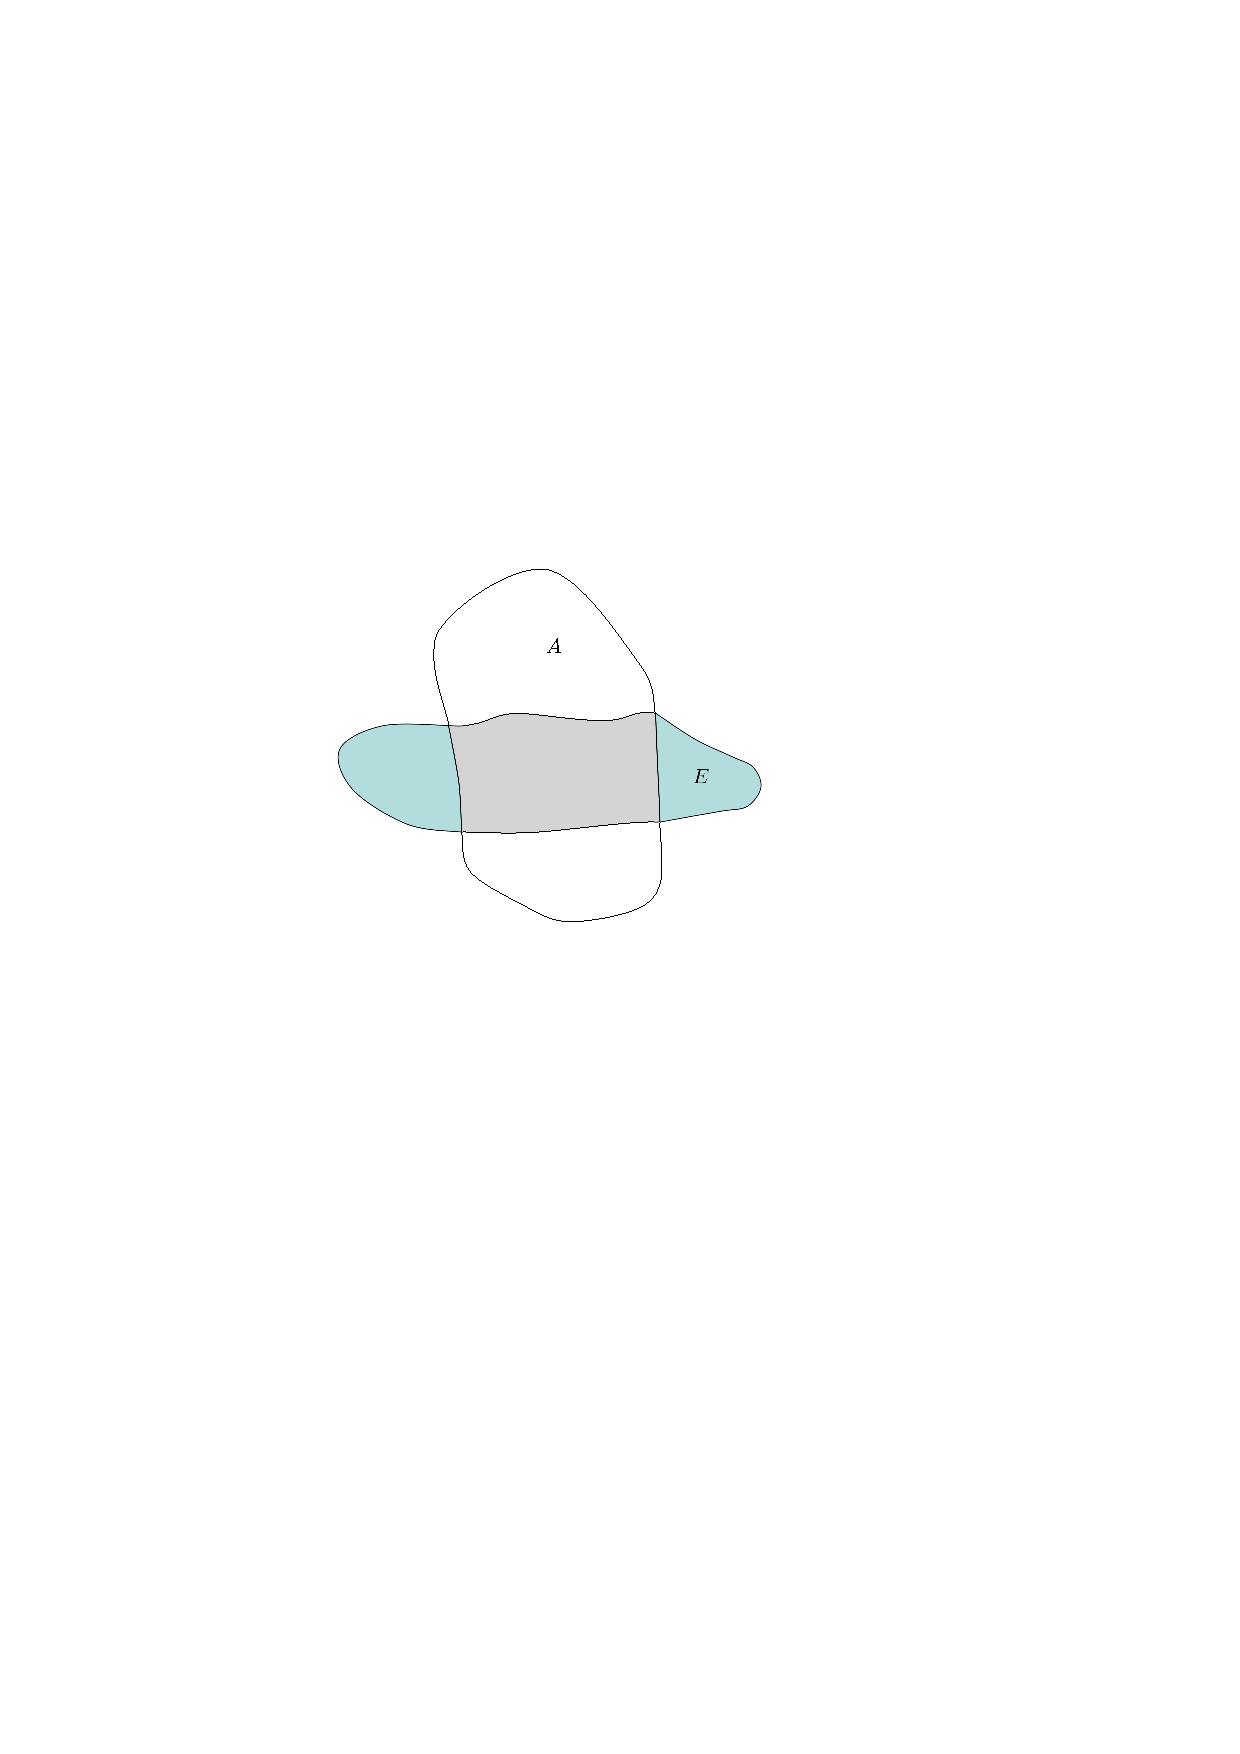
\includegraphics[width=0.3\textwidth]{MA4L11_1.png}
	\caption{Множество $A$ разбивает множество $E$.}
	\label{11_1}
\end{figure}
Очевидно, что $\VN \in \MA_\nu$, поскольку:
$$
	E \cap \VN = \VN, \, E \setminus \VN = E, \, \nu(E \cap \VN) + \nu(E\setminus \VN) = \nu(\VN) + \nu(E) = \nu(E)
$$
Аналогично, что $X \in \MA_\nu$, поскольку:
$$
	E \cap X = E, \, E \setminus X = \VN, \, \nu(E \cap X) + \nu(E\setminus X) = \nu(E) + \nu(\VN) = \nu(E)
$$
Какие ещё множества будут лежать в $\MA_\nu$? Множества меры нуль.
\begin{prop}
	Если $\nu(A) = 0$, то $A \in \MA_\nu$.
\end{prop}
\begin{proof}
	Возьмем произвольное $E$, тогда: 
	$$
		E \cap A \subset A \Rightarrow \nu(E \cap A) \leq \nu(A) = 0 \Rightarrow  \nu(E \cap A) = 0
	$$
	$$
		E \setminus A \subset E \Rightarrow \nu(E \setminus A) \leq \nu(E) \Rightarrow \nu(E\cap A) + \nu(E\setminus A)  \leq 0 +  \nu(E) \leq \nu(E\cap A) + \nu(E \setminus A) 
	$$
	где последнее неравенство следует из субаддитивности (свойство $3$ по определению). Тогда:
	$$
		\nu(E) = \nu(E\cap A) + \nu(E \setminus A)
	$$
\end{proof}

\textbf{Пример}: Рассмотрим наш предыдущий пример и попробуем понять из чего состоит $\MA_\nu$ там:
$$
	A \neq \VN \wedge A \neq X \Rightarrow X\setminus A \neq \VN \Rightarrow 1 = \nu(X) = \nu(A) + \nu(X \setminus A) = 1 + 1 
$$
Получили противоречие $\Rightarrow \MA_\nu = \{\VN, X\}$. В общем случае, объяснять какие множества относятся к $\MA_\nu$ это задача достаточно трудная даже на простых примерах.

\begin{theorem}(\textbf{теорема Каратеодори})
	$\MA_\nu$ это $\sigma$-алгебра и $\nu$ это $\sigma$-аддитивная мера на $\MA_\nu$.
\end{theorem}
\begin{rem}
	Теорема приводится без доказательства, доказательство можно посмотреть в книге Эванс, Гариеппи: теория меры и тонкие свойства функций (см. английскую версию).
\end{rem}
\begin{theorem}
	Пусть $X$ - метрическое пространство и $\nu$ - внешняя мера. Предположим, что верно:
	$$
		\forall A,B \subset X\colon \inf\limits_{a \in A, \, b \in B}\rho(a,b) > 0 \Rightarrow \nu(A \cup B) = \nu(A) + \nu(B)
	$$
	Тогда борелевские множества лежат в $\sigma$-алгебре измеримых множеств: $\MB(X) \subset \MA_\nu$.
\end{theorem}
\begin{rem}
	Теорема приводится без доказательства, доказательство можно посмотреть в книге Эванс, Гариеппи: теория меры и тонкие свойства функций.
\end{rem}

\subsection*{Мера Лебега}
Пусть $X = \MR^n$. Вопрос, как определяется внешняя мера? Она будет называться ``верхней мерой''.
\begin{defn}
	\uwave{Верхней мерой Лебега} называется функция на $X$:
	$$
		\lambda^*(E) = \inf\left\{\ddsum{j}{}|\MI_j|\; \bigg\vert \; \MI_j \text{ - замкнутые бруски}, \, E \subset \bigcup\limits_{j}\MI_j  \right\}
	$$
	где $\cup_j \MI_j$ это не более, чем счетное объединение замкнутых брусов.
\end{defn}
\begin{rem}
	Можно брать открытые брусы: раздуть или сжать.
\end{rem}
\begin{figure}[H]
	\centering
	\includegraphics[width=0.45\textwidth]{MA4L11_2.png}
	\caption{Покрытие множества $E$ не более, чем счетным объединением замкнутых брусов.}
	\label{11_2}
\end{figure}
Мы покрываем множество $E$ брусками (как угодно), но не более чем счетным количеством, затем считаем сумму объемов и берём точную нижнюю грань этих покрытий. Новизна здесь в том, чтобы покрывать счётным количеством брусков, а не каким-то (типа конечного набора). Единственное, что понять было сложно - есть ли аддитивность или $\sigma$-аддитивность.
\begin{rem}
	В действительном анализе внешняя мера определяется слегка по-другому: на произвольном измеримом пространстве, фиксировалась алгебра и верхней мерой объявлялась точная нижняя грань по счетным покрытиям элементами алгебры.
\end{rem}

\begin{rem}
	Заметим, что внешняя мера как раз взялась из определения выше. И мера Хаусдорфа и практически все внешние меры строятся похожим образом: выделяется класс множеств, на них вводятся функции (в данном случае - объем для параллелепипеда), а дальше устраиваете покрытие этими множествами и берёте точную нижнюю грань $\Rightarrow$ получаем некоторую внешнюю меру.
\end{rem}
\begin{rem}
	Заметим также, что определение внешней меры похоже на определение меры нуль по Лебегу. Отличие в том, что здесь мера не обязательно должна быть равна $0$, может получиться и $+\infty$.
\end{rem}
\begin{prop}
	$\lambda^*$ это внешняя мера и класс измеримых множеств содержит все борелевские множества, то есть: $\MB(\MR^n)\subset \MA_{\lambda^*}$.
\end{prop}
\begin{proof}
	Проверим, что $\lambda^*$ это внешняя мера:
	\begin{enumerate}[label=\arabic*)]
		\item $\lambda^*(\VN) = 0$, поскольку $\forall \VE > 0, \, \exists \, \MI \colon |\MI| < \VE, \, \VN \subset \MI$;
		\item Пусть $A \subset B$, где $B \subset \cup_j \MI_j$, тогда $A \subset \cup_j \MI_j \Rightarrow \lambda^*(A) \leq \sum_j |\MI_j|$ по определению $\lambda^*$. Следовательно, для любого покрытия $B$ имеем такое же неравенство $\Rightarrow \lambda^*(A)$ это просто какая-то нижняя грань, а $\lambda^*(B)$ это точная нижняя грань для всех таких покрытий $\Rightarrow$ по определению точной нижней грани получаем: $\lambda^*(A) \leq \lambda^*(B)$;
		\item Рассмотрим $\cup_m A_m$, тогда:
		$$
			\forall \VE > 0, \, \exists \, \MI_j^m \colon A_m \subset \bigcup\limits_j \MI_j^m \wedge \sum_j|\MI_j^m| \leq \lambda^*(A_m) + \dfrac{\VE}{2^m} 
		$$
		где последнее верно из определения точной нижней грани. Тогда:
		$$
			\bigcup\limits_m A_m \subset \bigcup\limits_{j,m}\MI_j^m \wedge \ddsum{j,m}{}|\MI_j^m|\leq \ddsum{m}{}\lambda^*(A_m) + \VE{\cdot}\ddsum{m}{}\dfrac{1}{2^m} \Rightarrow \lambda^*(\cup_m A_m) \leq \ddsum{m}{}\lambda^*(A_m) + \VE
		$$
		Устремляя $\VE$ к нулю, мы получаем требуемое равенство;
	\end{enumerate}
	Пусть $A$ и $B$ таковы, что:
	$$
		\exists \, \delta > 0 \colon \forall a \in A, b \in B,\, \|a - b\| \geq \delta
	$$
	Так как $\lambda^*$ это внешняя мера, то: $\lambda^*(A \cup B) \leq \lambda^*(A) + \lambda^*(B)$. Мы хотим доказать неравенство в обратную сторону и воспользуемся теоремой $2$ (критерий Каратеодори). Заметим, что в определении $\lambda^*$ можно считать, что все $\diam{\MI_j} < \tfrac{\delta}{3}$, поскольку мы можем разбить покрытие не более мелкое:
	$$
		E \subset \bigcup\limits_j \MI_j, \, \MI_j = \bigcup\limits_{k = 1}^{N_j} \MJ_k^j, \, \diam{\MJ_k^j} < \dfrac{\delta}{3}, \, \ddsum{k}{}|\MJ_k^j| = |\MI_j| \Rightarrow  E \subset \bigcup\limits_{j,k}\MJ_k^j \wedge \ddsum{k,j}{}|\MJ_k^j| = \ddsum{j}{}|\MI_j|
	$$
	Тогда взятие точной нижней грани по всем покрытиям параллелепипедами или параллелепипедами диаметра меньше $\tfrac{\delta}{3}$ совпадают $\Rightarrow \inf_{\MI_j} = \inf_{\MJ_k^j}$. Пусть теперь верно:
	$$
		A \cup B \subset \bigcup\limits_j \MI_j, \, \diam{\MI_j} < \dfrac{\delta}{3}, \, \ddsum{j}{}|\MI_j| \leq \lambda^*(A \cup B) + \VE
	$$
	где последнее опять верно в силу того, что $\lambda^*$ это точная нижняя грань. Если $\MI_j \cap (A \cup B) = \VN$, то такие множества - выбрасываем и далее считаем, что их нет. Не может быть ситуации:
	$$
		\MI_j \cap A \neq \VN \wedge \MI_j \cap B \neq \VN
	$$
	в противном случае, мы получим: $\forall a \in A, b \in B, \, \delta \leq \|a - b \| < \tfrac{\delta}{3} \Rightarrow$ противоречие. Тогда:
	$$
		\bigcup\limits_j \MI_j = \bigcup\limits_{j \colon \MI_j \cap A \neq \VN} \MI_j \sqcup  \bigcup\limits_{j \colon \MI_j \cap B \neq \VN} \MI_j \Rightarrow A \subset \bigcup\limits_{j \colon \MI_j \cap A \neq \VN} \MI_j \wedge B \subset \bigcup\limits_{j \colon \MI_j \cap B \neq \VN} \MI_j \Rightarrow
	$$
	$$
		\Rightarrow \ddsum{j}{}|\MI_j| = \ddsum{j \colon \MI_j \cap A \neq \VN}{}|\MI_j| \;\; + \ddsum{j \colon \MI_j \cap B \neq \VN}{}|\MI_j| \geq \lambda^*(A) + \lambda^*(B) \Rightarrow \VE + \lambda^*(A \cup B) \geq \lambda^*(A) + \lambda^*(B)
	$$
	Устремляя $\VE$ к нулю, мы получаем требуемое неравенство $\Rightarrow$ получаем требуемое равенство $\Rightarrow$ получаем по теореме $2$: $\MB(\MR^n) \subset \MA_{\lambda^*}$.
\end{proof}

Таким образом, $\lambda^*$ это $\sigma$-аддитивная мера на $\MA_{\lambda^*}$ (измеримое по Лебегу множество), где $\MB(\MR^n)\subset \MA_{\lambda^*}$ и далее $\lambda^*$ обозначаем просто $\lambda$ и называем \uwave{мерой Лебега}. Дополнительно, будем писать $\lambda_n$, если нам почему-то будет важно, что это на $\MR^n$. Множество измеримых по Лебегу будем писать, как $\MA_\lambda$. Теперь нам хотелось бы понять, как эта мера устроена.
\begin{prop}
	Пусть $\MI$ это замкнутый брус, тогда $\lambda(\MI)$ это объем $\MI$: $\lambda(\MI) = |\MI|$.
\end{prop}
\begin{proof}
	Брус покрыт самим собой $\Rightarrow \lambda(\MI) \leq |\MI|$. Возьмем любое покрытие $\MI$ открытыми брусками, тогда покрытие можно считать конечным (из компактности):
	$$
		\MI \subset \bigcup\limits_j \MI_j \Rightarrow \MI \subset \bigcup\limits_{m = 1}^{M} \MI_m \Rightarrow |\MI | \leq \ddsum{m = 1}{M}|\MI_j|
	$$
	где последнее следует из следствия $2$ лекции $1$ этого семестра. Тогда, поскольку это верно для произвольного покрытия, то это же будет верно и для точной нижней грани, то есть: $\lambda(\MI) \geq |\MI|$.
\end{proof}
\begin{rem}
	Внешние меры, которые строятся с помощью инфинумов, совершенно не обязаны продолжать то, с помощью чего мы считаем меры множеств, участвующих в покрытии.
\end{rem}
\begin{prop}
	$$
		E \subset \MA_\lambda \Leftrightarrow E = \bigcup\limits_m K_m \cup E_0 \Leftrightarrow E = B \cup B_0
	$$ 
	где $K_m$ это компакты, $E_0$ и $B_0$ это множества меры нуль и $B$ это борелевское множество.
\end{prop}
\begin{rem}
	Заметим, что не требуется, чтобы множества $E_0$ и $B_0$ совпадали.
\end{rem}
\begin{proof}\hfill
	\begin{enumerate}[label=\arabic*)]
		\item Покажем, что всякое борелевское множество $B$ можно представить в виде $B = \cup_m K_m \cup B_0$, где $K_m$ это компакты, $B_0$ это множество меры нуль. Можно считать, что $B \subset \MI$ - лежит в некотором замкнутом бруске, поскольку:
		$$
			\MR^n = \bigcup\limits_k \MI_k \Rightarrow B = \bigcup\limits_k (\MI_k \cap B)
		$$
		Следовательно, если каждое множество $\MI_k \cap B$ представить в виде объединения компактов и множества меры нуль, то можно и всё борелевское так представить. $\lambda$ это конечная $\sigma$-аддитивная мера на борелевских множествах на бруске: $\MB(\MI)$, тогда по теореме с прошлой лекции будет верно:
		$$
			\forall m, \, \exists \, F_m \subset B \colon \lambda(B \setminus F_m) < \dfrac{1}{m}
		$$
		$F_m$ это замкнутое множество, $F_m \subset B \subset \MI \Rightarrow F_m$ это компакт. Возьмем объединение $F_m$, тогда:
		$$
			\bigcup\limits_m F_m \subset B , \, B \setminus \bigcup\limits_m F_m \subset B \setminus F_m \Rightarrow \lambda(B \setminus \cup_m F_m) \leq \lambda(B \setminus F_m) < \dfrac{1}{m} \to 0
		$$
		Следовательно, получаем: 
		$$
			B = \bigcup\limits_m F_m \cup \left(B \setminus \bigcup\limits_m F_m\right)
		$$ 
		где $B \setminus \cup_m F_m$ это множество меры нуль;
		\item Заметим, что все стрелочки $\Leftarrow$ очевидны, поскольку борелевские множества - измеримы $\Rightarrow$ компакты измеримы, мы знаем, что множества меры нуль всегда измеримы (в самом начале обсуждения внешней меры проговорили) и также мы знаем, что множество измеримых это $\sigma$-алгебра $\Rightarrow$ всё что получаем счётным объединением это элемент этой $\sigma$-алгебры;
		\item По первому пункту достаточно доказать, что всякое измеримое множество есть объединение борелевского с множеством меры нуль (сделаем в следующий раз);
	\end{enumerate}
\end{proof}


\end{document}